% GENERATED by tools/render_sysml_diagrams.py. Do not edit: the next run overwrites it.
% To change a caption, edit the `// caption:` line above the view in the .sysml file.
% To explain a diagram, add `// note:` lines there; they follow the caption.
% To add or remove a figure, add or remove the view in the model.
% To move a figure between the body and the appendix, add or remove a
% `// placement: body` line above the caption line.

\begin{landscape}
\begin{figure}[!htbp]
\centering
\pdfimageresolution=300
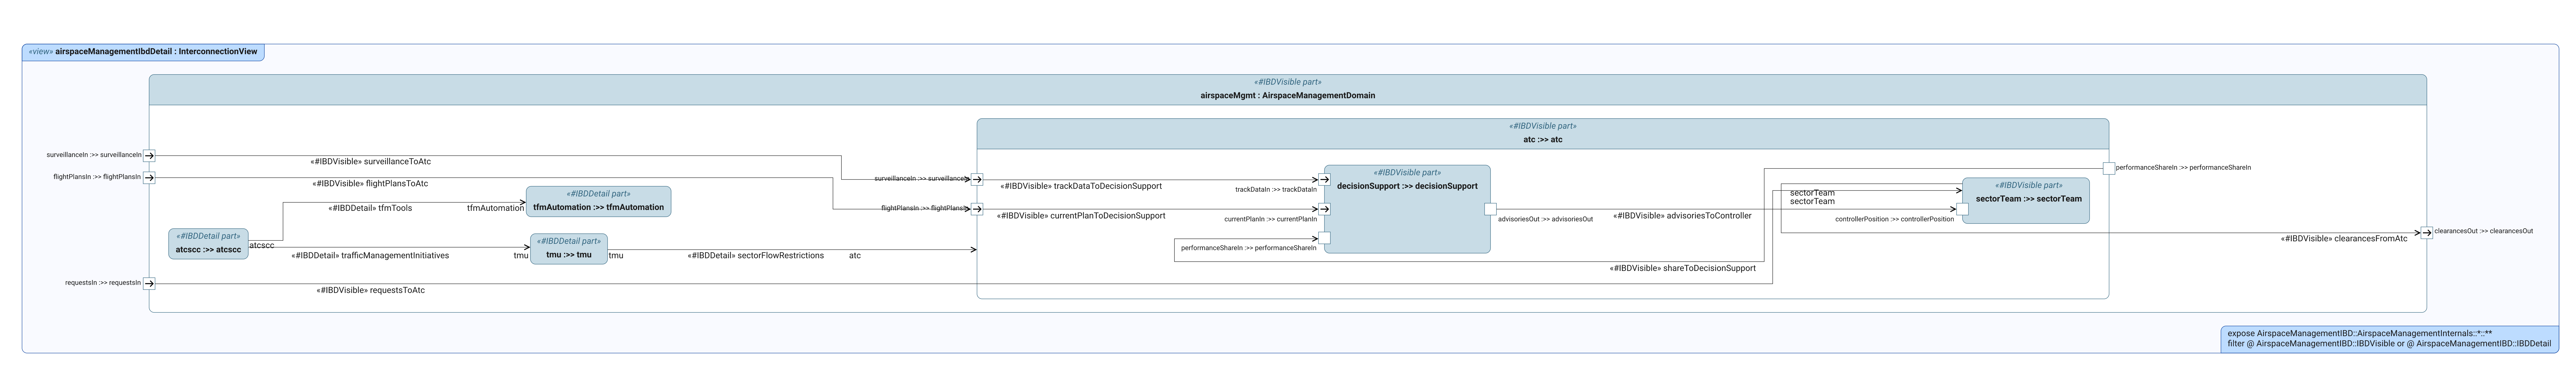
\includegraphics[width=\linewidth,height=0.8\textheight,keepaspectratio]{sysml/diagram-airspaceManagementIbdDetail}
\caption[Airspace management internal block diagram, detailed level: adds traffic flow management (the Command Center, the traffic management unit and the flow management tools)]{Airspace management internal block diagram, detailed level: adds traffic flow management (the Command Center, the traffic management unit and the flow management tools). ATC's decision support (decisionSupport : AtcDecisionSupport) is the En Route Decision Support Tool (EDST), the conflict probe in the en route automation (ERAM) that the sector controllers use (FAA JO 7110.65BB, para. 13-1-1). It is not a Command Center tool. Today EDST uses generic aircraft performance; the airline's performance share shown arriving at it is the proposed improvement, not part of today's system. View \texttt{airspaceManagementIbdDetail}; source \texttt{nas\_ibd\_airspace\_management.sysml}; rendered 2026-11-24.}
\label{fig:sysml-airspaceManagementIbdDetail}
\end{figure}
\end{landscape}
